\documentclass[a4paper,12pt]{article}
\usepackage[utf8]{inputenc}
\usepackage{graphicx}
\usepackage{fancyhdr}
\usepackage{amsmath}
\usepackage{adjustbox}
\usepackage{mathtools}
\usepackage{float}
\usepackage[spanish, es-nodecimaldot]{babel} 
\usepackage{lastpage}
\usepackage{amssymb} % Para símbolos matemáticos adicionales
\usepackage{hyperref}
\usepackage{cleveref}
%\usepackage[none]{hyphenat}
\usepackage{array}

\usepackage{multirow}
\usepackage{textcomp}
\usepackage[left=2.5cm, right=2.5cm, top=3cm, bottom=3cm]{geometry}

\graphicspath{{Imagenes/}}

% Encabezado y pie de página
\pagestyle{fancy}
\fancyhf{}
\setlength{\headheight}{30 pt}
\renewcommand{\headrulewidth}{0.2pt}
\fancyhead[R]{\begin{tabular}{@{}l@{}}
\includegraphics[scale=0.4]{escudo.PNG}\end{tabular}}
\fancyhead[L]{\begin{tabular}{@{}c@{}} \textbf{Robótica I - Año: 2024} \\ Trabajo Práctico 5: Cinemática Inversa \end{tabular}}


\fancyfoot[R]{\thepage}
\fancyfoot[C]{\begin{tabular}{@{}c@{}}\textbf{BORQUEZ PEREZ Juan Manuel}\\ \textbf{Legajo 13567}\end{tabular}}
\renewcommand{\footrulewidth}{0.2pt}

\begin{document}

\begin{titlepage}
    \centering
    \vspace*{5cm}
    {\Huge\bfseries Informe de Trabajo Práctico N°5}\\
    \vspace{0.2cm}
    {\Large \textbf{Cinemática Inversa}}\\
    \vspace{0.5cm}
    {\Large Robótica I}\\
    \vspace{0.5 cm}
    {\Large Ingeniería en Mecatrónica}\\
    \vspace{0.2 cm}
    {\Large Facultad de Ingeniería - UNCUYO}\\
    \vspace{1.5cm}
    Alumno: Juan Manuel BORQUEZ PEREZ\\
    Legajo: 13567\\
    \vfill
    {\begin{tabular}{@{}c@{}}
\includegraphics[scale=0.4]{escudo.PNG}\end{tabular}}\hspace{10pt}
    %Año 2023
\end{titlepage}

\section{Ejercicio 1}
\begin{figure}[H]
    \centering
    \begin{adjustbox}{scale = 0.55, max width=\columnwidth}
        \framebox{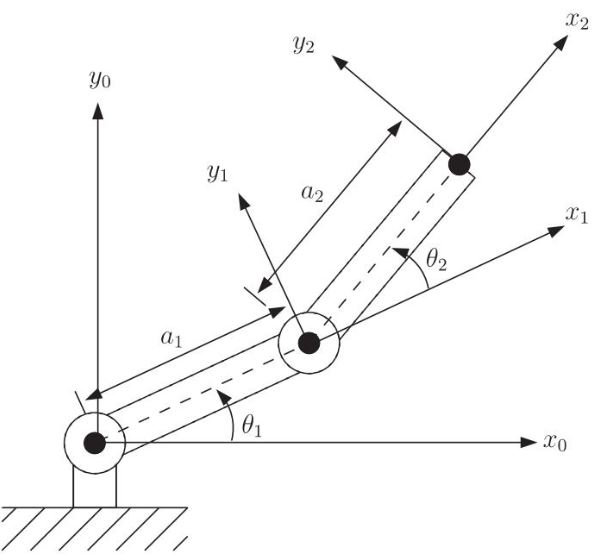
\includegraphics{1-Ejercicio_1.JPG}}
    \end{adjustbox}
    \caption{Robot Ejercicio 1}
\end{figure}

\subsection{}
\textbf{Utilice el método geométrico para hallar un conjunto de ecuaciones cerradas que resuelvan el siguiente problema}

\begin{equation*}
    \overline{q} = f\left(x,y,\gamma\right)
\end{equation*}

Al tratarse de un robot con solo dos grados de libertad, una \textbf{postura alcanzable está suficientemente definida al especificar
a lo sumo dos variables en el plano}, esto es, $\left(x,y\right)$, $\left(x,\gamma\right)$ o $\left(y, \gamma\right)$; mientras que
la tercera variable queda determinada. Luego, como el problema se formula en término de las tres variables, las mismas deben ser congruentes para
que exista solución.

Las posiciones alcanzables por el extremo del robot quedan definidas por las siguientes condiciones:
\begin{equation}
    \begin{aligned}
        \sqrt[]{x^2 + y^2 }&\leq  a_1 + a_2\,\,\, \text(extension\,maxima)\\
        \sqrt[]{x^2 + y^2} & \geq  |a_1 - a_2|\,\,\, \text(extesion\,minima)
    \end{aligned}
    \label{rango}
\end{equation}

Cuando la posición es alcanzable, $\theta_2$ se puede determinar por análisis de la suma de los vectores indicados en la \cref{geometria 1}, como se indica a continuación:
\begin{align*}
    \mathbf{w} &= \mathbf{u} + \mathbf{v}\\
    \mathbf{w}^2 &= \mathbf{u}^2 + \mathbf{v}^2 + 2\mathbf{u}\cdot\mathbf{v}\\
    x^2 + y^2 &= a_{1}^2 + a_{2}^2 + 2a_{1}a_{2}\cos(\theta_2)\\
\end{align*}
Luego:
\begin{equation}
    \theta_2 = arccos\left(\frac{x^2 + y^2 - a_{1}^2 - a_{2}^2}{2a_{1}a_{2}}\right)
    \label{teta2}
\end{equation}
Esto da lugar a \textbf{dos posibles valores}, uno positivo (codo abajo) y otro negativo (codo arriba).

\begin{figure}[htbp]
    \centering
    \begin{adjustbox}{scale = 0.55, max width=\columnwidth}
        \framebox{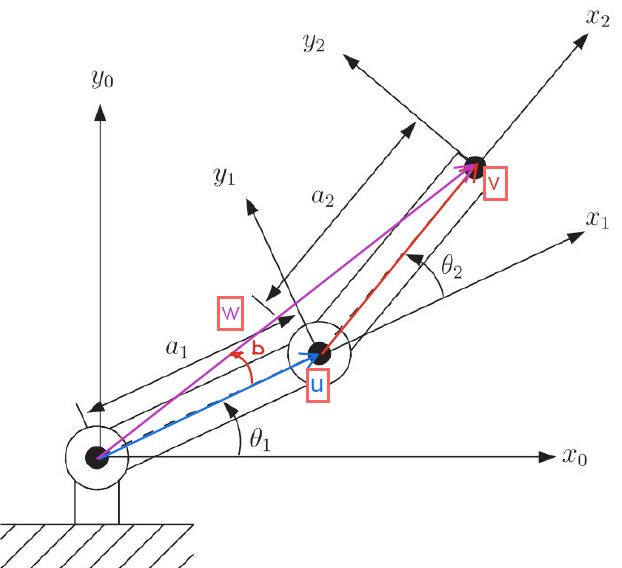
\includegraphics{2-Ejercicio_1_vectores.JPG}}
    \end{adjustbox}
    \caption{Análisis geométrico}
    \label{geometria 1}
\end{figure}

El ángulo $\theta_1$ se determina ahora por análisis de las proyecciones sobre los ejes

Sobre el eje X:
\begin{align*}
    x &= a_1\cos(\theta_1) + a_2\cos(\theta_1 + \theta_2)\\
    x &= a_1\cos(\theta_1) + a_2\left[\cos(\theta_1)\cos(\theta_2) - \sin(\theta_1)\sin(\theta_2)\right]\\
    x &= \underline{\left[a_1 + a_2\cos(\theta_2)\right]}\cos(\theta_1) - \underline{a_2\sin(\theta_2)}\sin(\theta_1)\\
    x &= \underline{A}\cos(\theta_1) - \underline{B}\sin(\theta_1)
\end{align*}
Sobre el eje Y:
\begin{align*}
    y &= a_1\sin(\theta_1) + a_2\sin(\theta_1 + \theta_2)\\
    y &= a_1\sin(\theta_1) + a_2\left[\sin(\theta_1)\cos(\theta_2) + \cos(\theta_1)\sin(\theta_2)\right]\\
    y &= \underline{\left[a_1 + a_2\cos(\theta_2)\right]}\sin(\theta_1) + \underline{a_2\sin(\theta_2)}\cos(\theta_1)\\
    y &= \underline{A}\sin(\theta_1) + \underline{B}\cos(\theta_1)
\end{align*}
Se obtiene el siguiente sistema de ecuaciones lineales:
\begin{align*}
    \begin{cases}
        x &= A\cos(\theta_1) - B\sin(\theta_1)\\
        y &= B\cos(\theta_1) + A\sin(\theta_1)
    \end{cases}
\end{align*}
Entonces se puede obtener $\theta_1$ a partir de las siguientes:
\begin{align}
    \begin{cases}
        \cos(\theta_1) &= \frac{Ax + By}{A^2 + B^2}\\
        \sin(\theta_1) &= \frac{Ay - Bx}{A^2 + B^2}\\
        \theta_1 &= \arctan{\left(\frac{Ay - Bx}{Ax + By}\right)}\\
        \theta_1 &=atan2(Ay-Bx, Ax + By)
    \end{cases}
    \label{teta1}
\end{align}
La tercera se utiliza para determinar dos posibles soluciones para $\theta_1$ mientras que el signo de las primeras dos determinan el valor correcto (el cuadrante).
En MATLAB se puede obtener el valor directamente como se indica en la cuarta condición, utilizando la función $atan2$.
La \cref{teta1} se resuelve para cada valor de B (uno por cada valor de $\theta_2$ dados en la \cref{teta2}).

Finalmente, la orientación dada para la postura en la formulación del problema debe ser congruente, y esta dada por:
\[\gamma = \theta_1 + \theta_2\]

Esta última condición, cuando se cumple permite acotar la solución a una sola del par obtenido.

En resumen, para $\overline{q} = (x, y, \gamma)$ en el rango del robot según \cref{rango} se obtiene un par de posibles soluciones (codo arriba y codo abajo) que luego se acota a una sola con la orientación:
\begin{align}
    \begin{cases}
        \theta_2 &= arccos\left(\frac{x^2 + y^2 - a_{1}^2 - a_{2}^2}{2a_{1}a_{2}}\right) \rightarrow A = a_1 + a_2\cos(\theta_2); B = a_2\sin(\theta_2)\\
        \theta_1 &=  atan2(Ay-Bx, Ax + By)\\
        \overline{q} &= (\theta_1, \theta_2)\\
        \text{solo\,si}\,\,\gamma &= \theta_1 + \theta_2
    \end{cases}
    \label{solucion ejercicio 1}
\end{align}
En este análisis consideramos que la formulación completa del problema debe ser congruente, es decir, $(x, y, \gamma)$ debe ser posible de obtener.
Sin embargo, \textbf{otra alternativa} podría ser exigir que \textbf{al menos dos de las variables en la formulación del problema sean congruentes} aunque la tercera no lo sea.
Así, por ejemplo, la posición podría estar fuera del alcance del robot porque la coordenada $y$ es demasiado grande, pero el par $(x, \gamma)$ ser congruente, en ese caso se obtiene una solución para este par y se descarta la restricción dada por $y$.
Para tomar en cuenta estas otras posibilidades, obtenemos a continuación soluciones del \textbf{problema a partir de $\mathbf{(x, \gamma)}$ o de $\mathbf{(y, \gamma)}$} cuando la otra coordenada de la posición se descarta.

\subsubsection{Formulación a partir de $(x, \gamma)$ o $(y, \gamma)$ cuando la otra no se toma en cuenta}
Volviendo a la \cref{geometria 1} tenemos:

\begin{align*}
    \mathbf{w} &= \mathbf{u} + \mathbf{v}\\
    \mathbf{w} - \mathbf{v} &= \mathbf{u}\\
    \left[x - a_2\cos(\gamma)\right]\mathbf{i} + \left[y - a_2\sin(\gamma)\right]\mathbf{j} &= \mathbf{u}\\
    \left[x - a_2\cos(\gamma)\right]^2 + \left[y - a_2\sin(\gamma)\right]^2 &= a_1^2\\
    |y - a_2\sin(\gamma)| &= \sqrt{a_1^2 - \left[x - a_2\cos(\gamma)\right]^2}\\
    ssi\,\,\{\Delta &= a_1^2 - \left[x - a_2\cos(\gamma)\right]^2\} >= 0
\end{align*}

Entonces, las condiciones para que exista solución del problema son:

\begin{align*}
    \left(x, \gamma\right)&\rightarrow\{\Delta_y = a_1^2 - \left[x - a_2\cos(\gamma)\right]^2\} >= 0\\
    \left(y, \gamma\right)&\rightarrow\{\Delta_x = a_1^2 - \left[y - a_2\sin(\gamma)\right]^2\} >= 0
\end{align*}

Cuando existe solución, se obtiene la coordenada faltante de la posición como:
\begin{align*}
    \left(x, \gamma\right)\rightarrow
    \begin{cases}
        y_1 &= \sqrt{\Delta_y} + a_2\sin(\gamma)\\
        y_2 &= -\sqrt{\Delta_y} + a_2\sin(\gamma)
    \end{cases}
    \\
    \left(y, \gamma\right)\rightarrow
    \begin{cases}
        x_1 &= \sqrt{\Delta_x} + a_2\cos(\gamma)\\
        x_2 &= -\sqrt{\Delta_x} + a_2\cos(\gamma)
    \end{cases}
\end{align*}

Así se llega a una formulación congruente del problema que se resuelve con la \cref{solucion ejercicio 1} en la que no hace falta verificar la orientación.



\subsection{}
\textbf{Utilice el método geométrico para hallar un conjunto de ecuaciones cerradas que resuelvan el siguiente problema}

\begin{equation*}
    \overline{q} = f\left(x,y\right)
\end{equation*}
La solución es la misma que en el caso anterior solamente que en este caso la orientación queda determinada por los desplazamientos angulares obtenidos:
\begin{align}
    \begin{cases}
        \theta_2 &= arccos\left(\frac{x^2 + y^2 - a_{1}^2 - a_{2}^2}{2a_{1}a_{2}}\right) \rightarrow A = a_1 + a_2\cos(\theta_2); B = a_2\sin(\theta_2)\\
        \theta_1 &=  atan2(Ay-Bx, Ax + By)\\
        \overline{q} &= (\theta_1, \theta_2)
    \end{cases}
\end{align}

\subsection{}
\textbf{Indique la cantidad de soluciones posibles que tendría cada conjunto de ecuaciones anterior, si los límites articulares fueran los siguientes}
\subsubsection{$\pm 90^\circ$}
La mínima extensión alcanzable por el robot se consigue cuando los eslabones forman un ángulo recto. Luego la condición de rango señalada en \cref{rango} es ahora:
\begin{equation}
    \begin{aligned}
        \sqrt{x^2 + y^2}&\leq  a_1 + a_2\,\,\, \text(extension\,maxima)\\
        x^2 + y^2& \geq a_1^2 + a_2^2\,\,\, \text(extension\,minima)
    \end{aligned}
    \label{rango 90}
\end{equation}

Para los puntos dentro del rango del robot, definido en \cref{rango 90}, se tendrá:
\begin{itemize}
    \item Para la ecuación 1, una sola solución posible para cada $\left(x, y, \gamma\right)$ válido.
    \item Para la ecuación 2, en general dos soluciones en el cuadrante 1 y 4 (codo arriba y codo abajo), excepto en los extremos del espacio de trabajo del robot cerca del cuadrante 2 y 3 en donde una de las soluciones ponga fuera de límite a la variable $q_1$, en esos casos solo es una sola solución. También hay una sola solución en las extensiones máximas.
\end{itemize}

\subsubsection{$\pm 180^\circ$}

\begin{itemize}
    \item Para la ecuación 1, en general, una sola solución posible para cada $\left(x, y, \gamma\right)$ válido. Dos soluciones para cada punto en la mínima extensión ($\theta_2 = \pm 180^\circ$). Dos soluciones cuando el punto está en la máxima extensión a $180^\circ$ del eje x ($q_1 = \pm 180^\circ$). Cuatro soluciones cuado el punto se encuentra en la mínima extensión a $180^\circ$ del eje x ($q_1, q_2 = \pm 180^\circ$).
    \item Para la ecuación 2, dos soluciones (codo arriba y codo abajo) más el caso particular de cuatro soluciones para la ecuación 1. Una sola solución en las extensines máximas.
\end{itemize}

\subsubsection{$\pm 225^\circ$}

\begin{itemize}
    \item Para la ecuación 1 en general una solución para puntos no tan cercanos al límite inferior del rango del robot (puntos en donde el segundo eslabon no se encuentre tan replegado), en zonas entre los $135^\circ$ y $-135^\circ$ respecto del eje x (del lado del eje x positivo), en cambio, se pueden obtener dos soluciones cuando los puntos están entre $135^\circ$ y $-135^\circ$ respecto del eje x (del lado del eje x negativo) dado que son alcanzables con giros positivos y negativos en la primera articulación. Cuando
    el eslabón 2 está lo suficientemente replegado (puntos cerca del límite inferior del rango del robot) también se puede alcanzar la postura con un giro positivo y un giro negativo en la segunda articulación y habrán dos soluciones. En este último caso, cuando además la posición se encuentra entre $135^\circ$ y $-135^\circ$ respecto del eje x (del lado del eje x negativo) tendremos hasta cuatro soluciones (un giro positivo y negativo por cada articulación).
    \item Para la ecuación 2 ahora además existen dos posibilidades (codo arriba y codo abajo) para cada caso. Luego existen dos soluciones cuando los puntos no están cerca del límite mínimo del rango y no se encuentran en la región de solapamiento del rango articular de la primera articulación. Cuatro soluciones en los puntos que se encuentran en la región de solapamiento del rango articular de la primera articulación y que no están cerca del mínimo del rango del robot. Cuatro soluciones en puntos que no están en la zona de solapamiento de la primera articulación y están cerca del mínimo del rango del robot. Ocho soluciones cuando los puntos se encuentra cerca el mínimo del rango y en la región de solapamiento articular de la primera articulación. Una única solución en la máxima extensión en la región de no solapamiento. Dos soluciones en la máxima extensión en la región de solapamiento. Dos soluciones en la mínma extensión en la zona de no solapamiento. Cuatro soluciones en la mínima extensión en la zona de solapamiento.
\end{itemize}

\subsubsection{$\pm \infty$}
Infinitas soluciones para ambas ecuaciones.

\section{Ejercicio 2}
\textbf{Analice los 3 robots que se muestran a continuación y plantee el problema de
cinemática inversa de la forma $\overline{q} = f(...)$ de una forma que implique infinitas soluciones, y de
otra que implique un número finito de soluciones. Considere límites de $\pm 180^\circ$ para
articulaciones rotacionales y $\pm\infty$ para las prismáticas.}
\subsection{}
\begin{figure}[H]
    \centering
    \begin{adjustbox}{scale = 0.55, max width=\columnwidth}
        \framebox{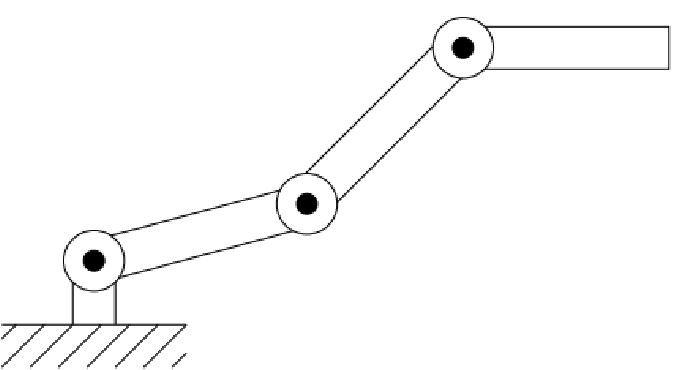
\includegraphics{3-Ejercicio_2_robot_RRR.JPG}}
    \end{adjustbox}
    \caption{Ejercicio 2.1}
\end{figure}

Exceptuando aquellos puntos que se encuentran en los extremos del alcance del robot, la siguiente formulación del problema
tiene \textbf{infinitas soluciones} para puntos alcanzables:

\begin{equation*}
    \overline{q} = f(x, y)
\end{equation*}

La siguiente formulación da un \textbf{número finito de soluciones}, a lo sumo dos (codo arriba y codo abajo).
\begin{equation}
    \overline{q} = f(x, y, \gamma)
    \label{problema RRR}
\end{equation}

\subsection{}
\begin{figure}[H]
    \centering
    \begin{adjustbox}{scale = 0.55, max width=\columnwidth}
        \framebox{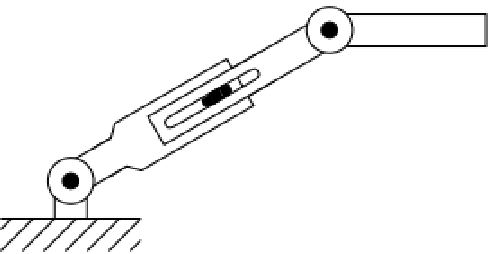
\includegraphics{4-Ejercicio_2_robot_RLR.JPG}}
    \end{adjustbox}
    \caption{Ejercicio 2.2}
\end{figure}


La siguiente formulación del problema da \textbf{infinitas soluciones}:
\begin{equation*}
    \overline{q} = f(x, y)
\end{equation*}

La siguiente formulación a una \textbf{solución única al problema}:
\begin{equation*}
    \overline{q} = f(x, y, \gamma)
\end{equation*}

\subsection{}
\begin{figure}[H]
    \centering
    \begin{adjustbox}{scale = 0.55, max width=\columnwidth}
        \framebox{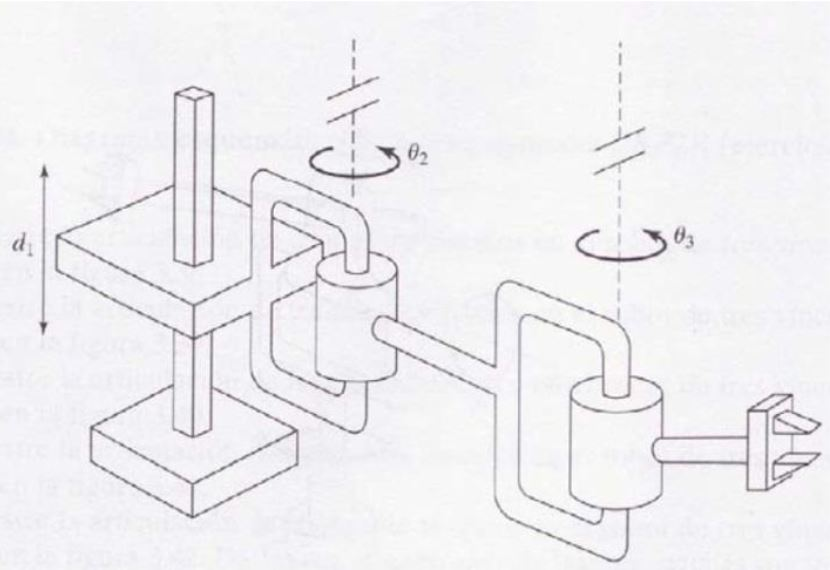
\includegraphics{5-Ejercicio_2_robot_LRR.JPG}}
    \end{adjustbox}
    \caption{Ejercicio 2.3}
\end{figure}

La siguiente formulación del problema da \textbf{infinitas soluciones} dado que se puede alcanzar una misma posición en el plano a diferentes elevaciones:
\begin{equation*}
    \overline{q} = f(x, y)
\end{equation*}

La siguiente formulación da \textbf{múltiples soluciones} (codo arriba y codo abajo en el plano xy):
\begin{equation}
    \overline{q} = f(x, y, z)
    \label{problema robot 3.2}
\end{equation}

La siguiente formulación da \textbf{una única solución} a lo sumo:
\begin{equation*}
    \overline{q} = f(x, y, z, \gamma)
\end{equation*}

Acá se toma en cuenta que \textbf{en cualquier postura válida, los ángulos de roll y pitch serán nulos}, con lo cual no se toman en cuenta en la formulación del problema.

\section{Ejercicio 3}
\textbf{Halle un conjunto de ecuaciones cerradas que resuelvan el problema
cinemático inverso del robot 2.2 por el método geométrico. Seleccione una formulación con
cantidad finita de soluciones. Establezca la cantidad de soluciones y analice si es necesario
contemplar límites finitos en la segunda articulación.}

\begin{figure}[H]
    \centering
    \begin{adjustbox}{scale = 0.55, max width=\columnwidth}
        \framebox{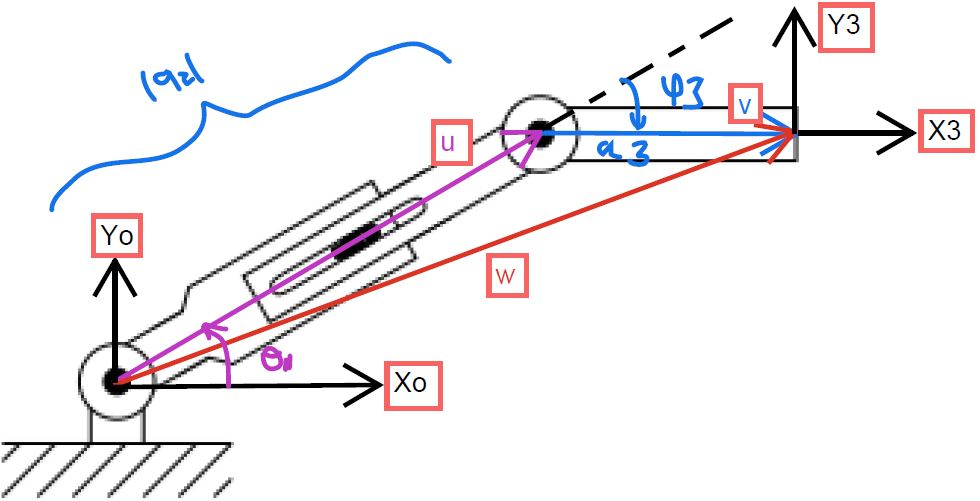
\includegraphics{6-Ejercicio_3_robot_RLR.JPG}}
    \end{adjustbox}
    \caption{Análisis geométrico}
\end{figure}

Se busca:
\begin{equation*}
    \overline{q} = f(x, y, \gamma)
\end{equation*}
En donde ahora $\gamma$ es el ángulo que forma el eje $X$ de $\{S_3\}$ respecto del eje X del sistema $\{S_O\}$.

Por un lado tenemos:
\begin{align*}
    \mathbf{w} &= \mathbf{u} + \mathbf{v}\\
    \mathbf{u} &= \mathbf{w} - \mathbf{v}\\
    u_x\mathbf{i} + u_y\mathbf{j} &= x\mathbf{i} + y\mathbf{j} - a_3\cos(\gamma)\mathbf{i} - a_3\sin(\gamma)\mathbf{j}
\end{align*}
Y por otro lado:
\begin{equation*}
    \gamma = \theta_1 + \theta_3
\end{equation*}
Luego, se puede obtener:
\begin{align*}
    u_x &= x - a_3\cos(\gamma)\\
    u_y &= y - a_3\sin(\gamma)\\
    \theta_1 &= atan2(u_y, u_x)\\
    \theta_3 &= \gamma - \theta_1\\
    |q_2| &= \sqrt{u_x^2 + u_y^2}
\end{align*}
Si se considera que el rango en la segunda articulación es $\pm \infty$, en realidad, la solución podría ser $\theta_1$ y su suplemento en el otro sentido y de la misma manera para $\theta_3$, pudiendo además ser $q_2$ el valor calculado y su opuesto.
Si, en cambio, se toma el \textbf{rango de la segunda articulación como $0-\infty$}, entonces la solución puede expresarse como:

\begin{align}
    \begin{cases}
        \theta_1 &= atan2(y - a_3\sin(\gamma), x - a_3\cos(\gamma))\\
        \theta_3 &= \gamma - \theta_1\\
        q_2 &= \sqrt{\left[x - a_3\cos(\gamma)\right]^2 + \left[y - a_3\sin(\gamma)\right]^2}
    \end{cases}
\end{align}

\section{Ejercicio 4}
\textbf{Trabaje con el robot 2.3 y halle un conjunto de ecuaciones que resuelvan la
cinemática inversa por el método algebraico. Se recomienda usar un software que permita el
trabajo simbólico.}

Para este robot consideramos la definición de los sistemas de referencia articulares que se tomó para el \textbf{Ejercicio 2.3} en el \textbf{``Trabajo Práctico 3: Denavit-Hartenberg''} como se muestra a continuación:
\begin{figure}[H]
    \centering
    \begin{adjustbox}{scale = 0.66, max width=\columnwidth}
        \framebox{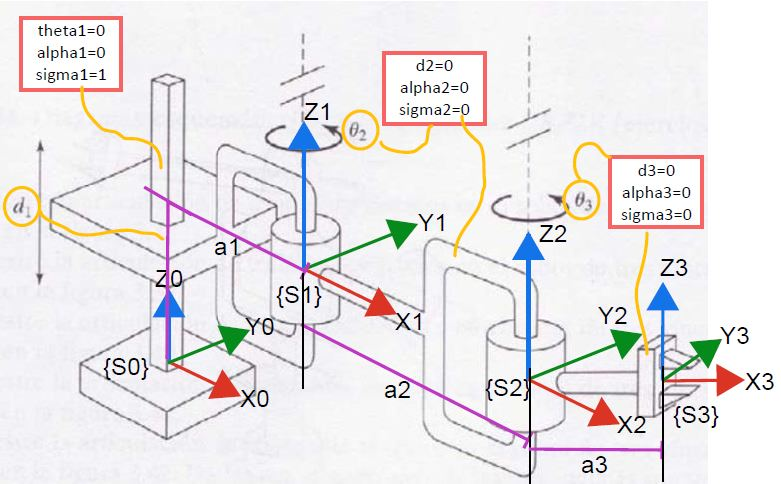
\includegraphics{7-Ejercicio_2_3_DH.JPG}}
    \end{adjustbox}
    \caption{Definición de sistemas Ejercicio 2.3 TP N°3}
\end{figure}

Los parámetros DH correspondientes son:
\begin{table}[H]
    \centering
    \begin{tabular}{|c|c|c|c|c|c|}
    \hline
    Sistema & $\theta$  & $d$ & $a$         & $\alpha$ & $\sigma$ \\ \hline
    1       & $0$       & $q_1$ & $a_{1}$  & 0      & 1        \\ \hline
    2       & $q_2$     & 0   & $a_{2}$  & 0        & 0        \\ \hline
    3       & $q_3$     & 0   & $a_{3}$  & 0        & 0        \\ \hline
    \end{tabular}
    \caption{Síntesis de la convención DH Ejercicio 2.3 TP N°3.}
\end{table}

Se considera la formulación del problema dada en \cref{problema robot 3.2}.

Se implementa un código en MATLAB en el archivo ``Ejercicio\_4.m'' en donde se obtiene la matriz de transformación homogénea para la cinemática directa del robot dadas coordenadas articulares genéricas como $\overline{q} = \left[q_1\, q_2\, q_3\right]$.

\begin{equation}
    CD = \left(\begin{array}{cccc} \cos\left(q_{2}+q_{3}\right) & -\sin\left(q_{2}+q_{3}\right) & 0 & a_{1}+a_{3}\,\cos\left(q_{2}+q_{3}\right)+a_{2}\,\cos\left(q_{2}\right)\\ \sin\left(q_{2}+q_{3}\right) & \cos\left(q_{2}+q_{3}\right) & 0 & a_{3}\,\sin\left(q_{2}+q_{3}\right)+a_{2}\,\sin\left(q_{2}\right)\\ 0 & 0 & 1 & q_{1}\\ 0 & 0 & 0 & 1 \end{array}\right)
    \label{CD generica}
\end{equation}

La anterior se iguala a una postura problema para la que se quieran obtener las coordenadas articulares, la cual está dada a partir de su matriz de transformación homogénea $T$ como.

\begin{equation}
    T = \left(\begin{array}{cccc} \cos\left(\mathrm{\gamma}\right) & -\sin\left(\mathrm{\gamma}\right) & 0 & x\\ \sin\left(\mathrm{\gamma}\right) & \cos\left(\mathrm{\gamma}\right) & 0 & y\\ 0 & 0 & 1 & z\\ 0 & 0 & 0 & 1 \end{array}\right)
    \label{postura}
\end{equation}

En donde se toma en cuenta que los ángulos de roll y pitch deben ser nulos.
De la igualdad elemento a elemento de las matrices $CD$ y $T$, eliminando las ecuaciones repetidas y aquellas que implican alguna restricción dada por $\gamma$ (la que no se exige según la formulación considerada del problema), se puede obtener el siguiente sistema de ecuaciones.

\begin{align}
    \begin{cases}
        a_1 + a_3cos(q_2 + q_3) + a_2cos(q_2) &= x\\
        a_3\sin(q_2 + q_3) + a_2\sin(q_2) &= y\\
        q_1 &= z
    \end{cases}
    \label{postura}
\end{align}

\begin{align*}
    \begin{cases}
        q_1 &= z\\
        q_2 &=  2\,\mathrm{atan}\left(\frac{2\,a_{2}\,y+\sqrt{-{a_{2}}^4+2\,{a_{2}}^2\,{a_{3}}^2+2\,{a_{2}}^2\,\overline{x}^2+2\,{a_{2}}^2\,y^2-{a_{3}}^4+2\,{a_{3}}^2\,\overline{x}^2+2\,{a_{3}}^2\,y^2-\overline{x}^4-2\,\overline{x}^2\,y^2-y^4}}{{a_{2}}^2+2\,a_{2}\,\overline{x}-{a_{3}}^2+\overline{x}^2+y^2}\right)\\
        q_3 &= -2\,\mathrm{atan}\left(\frac{\sqrt{\left(-{a_{2}}^2+2\,a_{2}\,a_{3}-{a_{3}}^2+\overline{x}^2+y^2\right)\,\left({a_{2}}^2+2\,a_{2}\,a_{3}+{a_{3}}^2-\overline{x}^2-y^2\right)}}{-{a_{2}}^2+2\,a_{2}\,a_{3}-{a_{3}}^2+\overline{x}^2+y^2}\right)
    \end{cases}
\end{align*}
\begin{align*}
    \begin{cases}
        q_1 &= z\\
        q_2 &= 2\,\mathrm{atan}\left(\frac{2\,a_{2}\,y-\sqrt{-{a_{2}}^4+2\,{a_{2}}^2\,{a_{3}}^2+2\,{a_{2}}^2\,\overline{x}^2+2\,{a_{2}}^2\,y^2-{a_{3}}^4+2\,{a_{3}}^2\,\overline{x}^2+2\,{a_{3}}^2\,y^2-\overline{x}^4-2\,\overline{x}^2\,y^2-y^4}}{{a_{2}}^2+2\,a_{2}\,\overline{x}-{a_{3}}^2+\overline{x}^2+y^2}\right)\\
        q_3 &= 2\,\mathrm{atan}\left(\frac{\sqrt{\left(-{a_{2}}^2+2\,a_{2}\,a_{3}-{a_{3}}^2+\overline{x}^2+y^2\right)\,\left({a_{2}}^2+2\,a_{2}\,a_{3}+{a_{3}}^2-\overline{x}^2-y^2\right)}}{-{a_{2}}^2+2\,a_{2}\,a_{3}-{a_{3}}^2+\overline{x}^2+y^2}\right)
    \end{cases}
\end{align*}

En las que se toma:
\begin{align*}
    \overline{x} = x-a_1
\end{align*}

\section{Ejercicio 5}
\textbf{Implemente las ecuaciones de cinemática inversa del robot 2.1 en un
script de Matlab aislado. La implementación debe resolver el problema entregando todos los
posibles vectores de solución en el espacio articular, considerando límites articulares de
$\pm180^\circ$.}

\textbf{Considere que el ejercicio será aprobado cuando se puedan obtener resultados correctos al
variar los parámetros de entrada.}

Se considera la definición de los sistemas de referencia y la aplicación de la convención de DH dada para el mismo robot en el TP N° 3.

\begin{figure}[H]
    \centering
    \begin{adjustbox}{scale = 0.58, max width=\columnwidth}
        \framebox{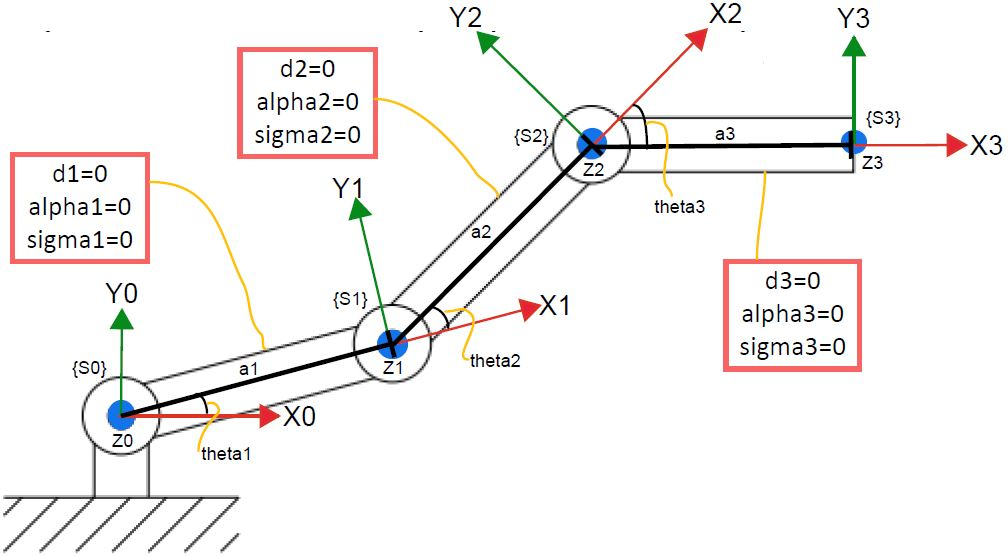
\includegraphics{8-Ejercicio_5_DH.JPG}}
    \end{adjustbox}
    \caption{Aplicación de la convención DH.}
\end{figure}

\begin{table}[H]
    \centering
    \begin{tabular}{|c|c|c|c|c|c|}
    \hline
    Sistema & $\theta$ & $d$ & $a$         & $\alpha$ & $\sigma$ \\ \hline
    1       & $q_1$     & 0   & $a_{1}$  & 0        & 0        \\ \hline
    2       & $q_2$     & 0   & $a_{2}$  & 0        & 0        \\ \hline
    3       & $q_3$     & 0   & $a_{3}$  & 0        & 0        \\ \hline
    \end{tabular}
    \caption{Convención DH robot 2.1}
\end{table}

El problema se formula como en \cref{problema RRR}.

La cinemática inversa de este robot \textbf{se puede resolver aplicando algo similar al paso inicial en el método del desacople cinemático de Pieper}.

Como se conoce la posición del extremo y la orientación del último eslabón , \textbf{se puede determinar la posición del extremo del segundo eslabón} $\prescript{O}{}{p_2} = (\prescript{O}{}{x_2}, \prescript{O}{}{y_2})$ como:
\begin{align*}
    \prescript{O}{}{p_2} &= \prescript{O}{}{p_3} - \mathbf{w}\\
    \prescript{O}{}{x_2}\mathbf{i} + \prescript{O}{}{y_2}\mathbf{j} &= \prescript{O}{}{x_3}\mathbf{i} + \prescript{O}{}{y_3}\mathbf{j} - \left(a_3\cos(\gamma)\mathbf{i} + a_3\sin(\gamma)\mathbf{i}\right)\\
\end{align*}
Luego
\begin{align*}
    \begin{cases}
        \prescript{O}{}{x_2} &= \prescript{O}{}{x_3} - a_3\cos(\gamma)\\
        \prescript{O}{}{y_2} &= \prescript{O}{}{y_3} - a_3\sin(\gamma)
    \end{cases}
\end{align*}
Esta, está \textbf{solo determinada por las variables articulares $q_1$ y $q_2$}, y encontrar sus valores dado $\prescript{O}{}{p_2}$ \textbf{es el problema de la cinemática inversa del robot del Ejercicio 1}.

Finalmente el valor de $q_3$ se obtiene por:
\[
    q_1 + q_2 + q_3 = \gamma
\]

\section{Ejercicio 6}
\textbf{Aplicación de método numérico. Trabaje con el LBR iiwa 7 R800 (KUKA). Explore la
función ``SerialLink/ikine'' del toolbox de Peter Corke y experimente con los parámetros de la
misma (vector semilla, iteraciones, tolerancia, etc.) para hallar al menos 3 soluciones de CI
para la siguiente posición y orientación del extremo final}

\begin{equation*}
    T = 
    \begin{bmatrix}
        1 & 0 & 0 & 0.23\\
        0 & 1 & 0 & 0.70\\
        0 & 0 & 1 & 0.60\\
        0 & 0 & 0 & 1
    \end{bmatrix}
\end{equation*}




%\begin{equation*}
%    \prescript{O}{}{Rot_M} = 
%    \begin{bmatrix}
%        0.500 & -0.866\\
%        0.866 & 0.500
%    \end{bmatrix}
%\end{equation*}

%\begin{figure}[H]
%    \centering
%    \begin{adjustbox}{scale = 0.85, max width=\columnwidth}
%        \framebox{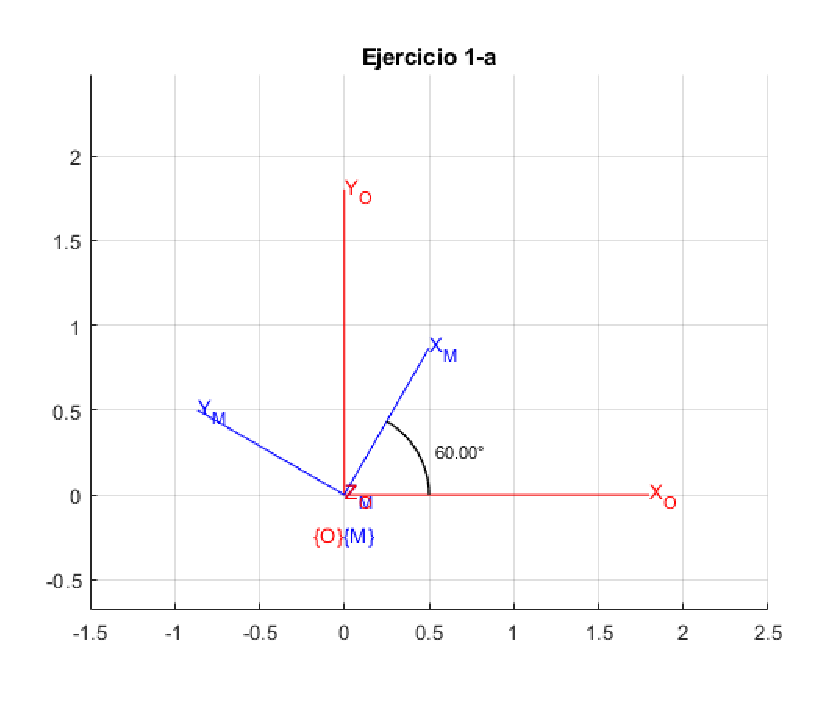
\includegraphics{1-Ejercicio_1_a.pdf}}
%    \end{adjustbox}
%    \caption{Sistema O y Sistema M superpuestos con indicación de ángulo de rotación.}
%\end{figure}


%\begin{table}[H]
%    \centering
%    \begin{tabular}{|c|c|c|c|c|c|}
%    \hline
%    Sistema & $\theta$  & $d$           & $a$    & $\alpha$ & $\sigma$ \\ \hline
%    1       & $q_1$     & $199.2$       & $200$  & 0        & 0        \\ \hline
%    2       & $q_2$     & $59.5$        & $250$  & 0        & 0        \\ \hline
%    3       & $0$       & $q_3$         & $0$    & 180°     & 1        \\ \hline
%    4       & $q_4$     & $37.5$        & $0$    & 0        & 0        \\ \hline
%    \end{tabular}
%    \caption{Parámetros DH alternativos.}
%    \label{parametros DH2}
%\end{table}

\end{document}